\chapter{Acoustic measurements}

\newpage
\begin{figure}[H]
    \centering
    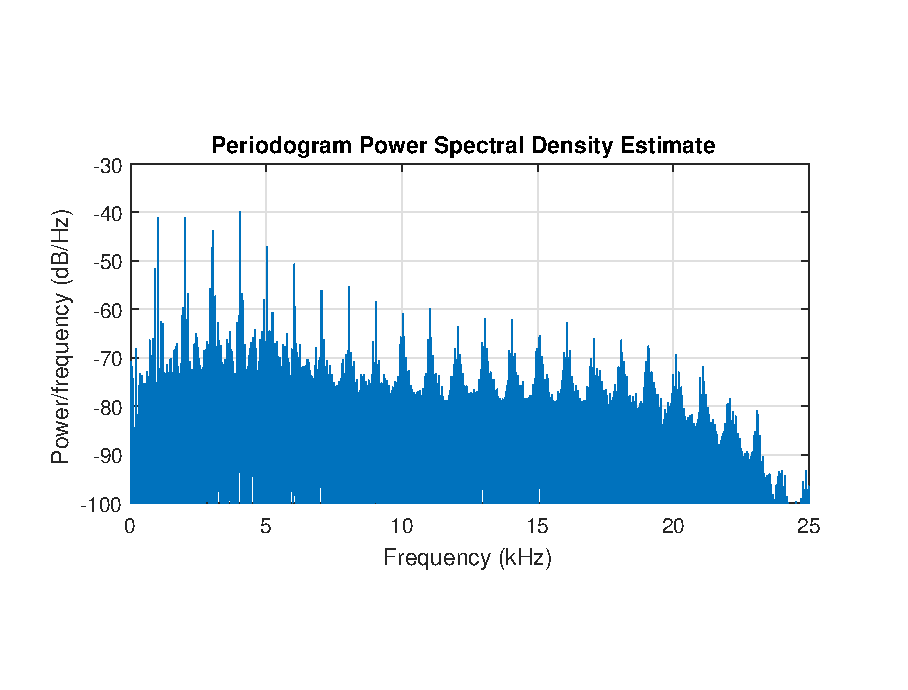
\includegraphics[trim={0cm 1.6cm 0cm 2cm},clip,width=\textwidth]{img/Periodogram_1khz-09.eps}
    \caption{Periodogram of 1kHz recorded tone, duty cycle 09.}
    \label{fig:appdx:period_1k-09}
\end{figure}
\begin{figure}[H]
    \centering
    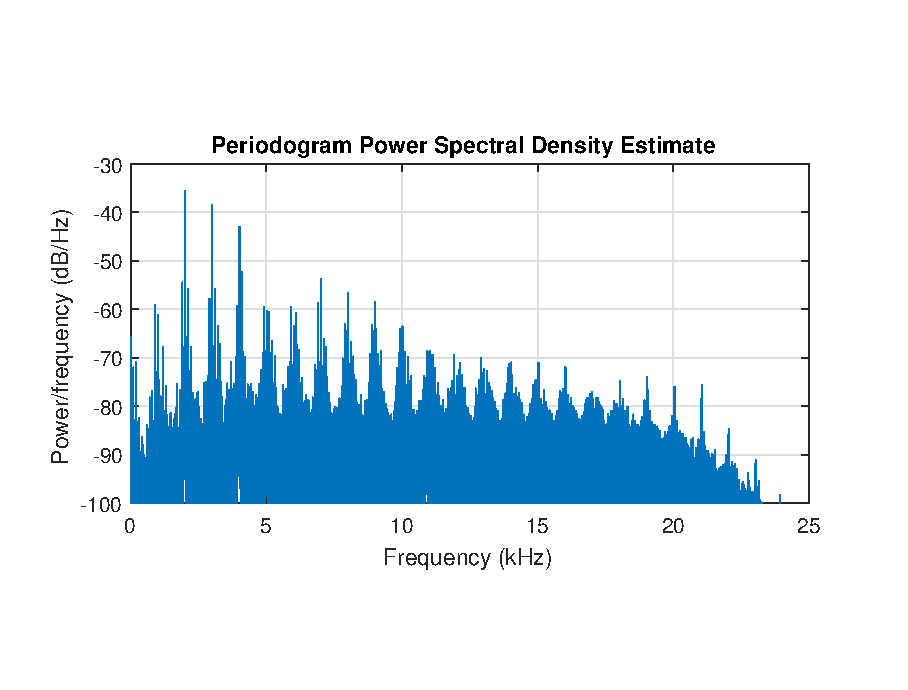
\includegraphics[trim={0cm 1.6cm 0cm 2cm},clip,width=\textwidth]{img/akustisk/Periodogram_1kHz-10.eps}
    \caption{Periodogram of 1kHz recorded tone, duty cycle 10.}
    \label{fig:appdx:period_1k-10}
\end{figure}

\begin{figure}[H]
    \centering
    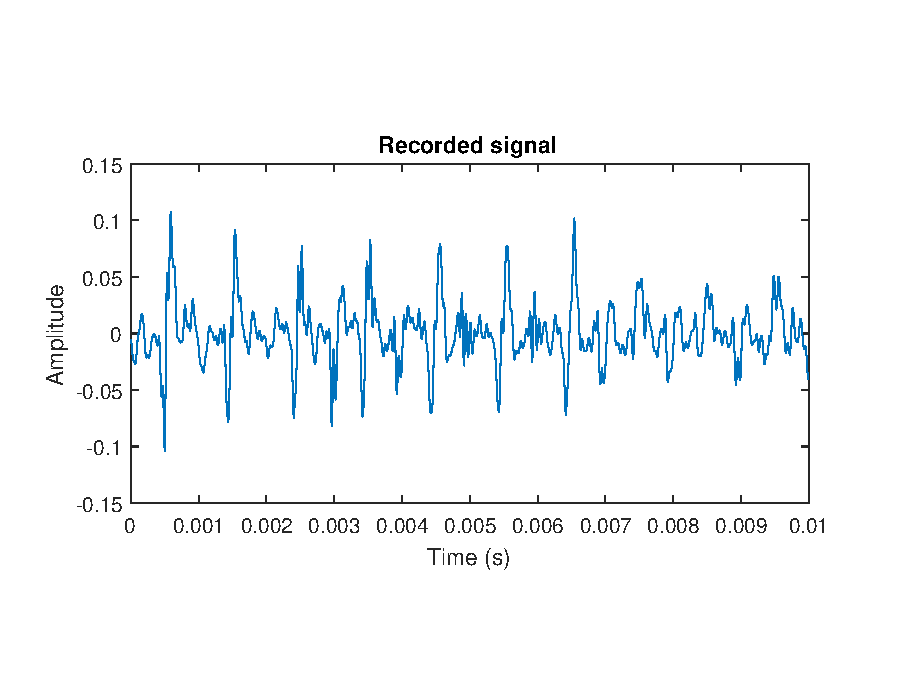
\includegraphics[trim={0cm 1.6cm 0cm 2cm},clip,width=\textwidth]{img/Recorded_1khz-09.eps}
    \caption{Time domain plot of 1kHz recorded tone, duty cycle 09.}
    \label{fig:appdx:wave_1k-09}
\end{figure}
\begin{figure}[H]
    \centering
    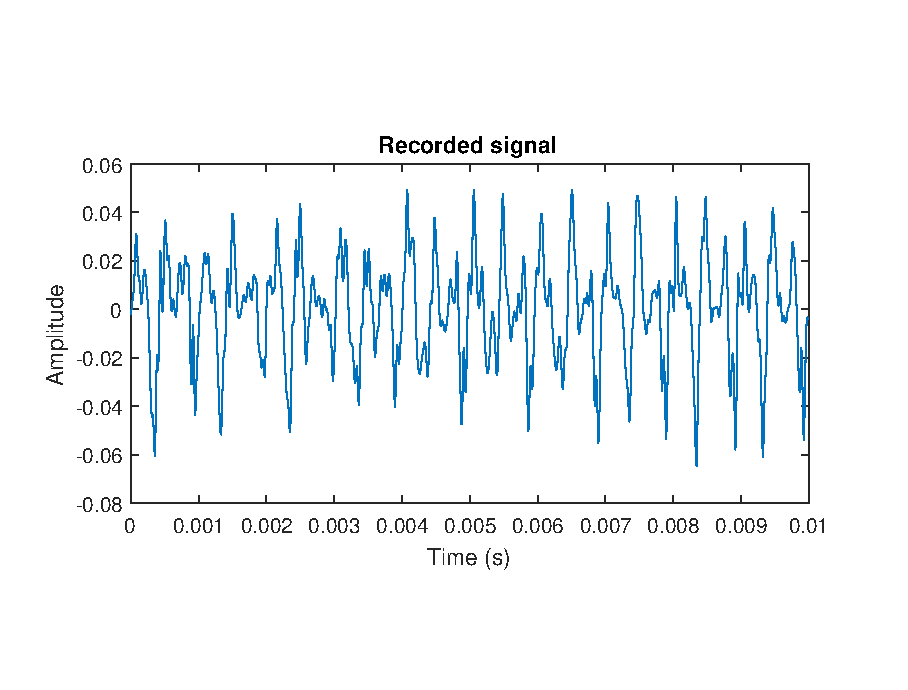
\includegraphics[trim={0cm 1.6cm 0cm 2cm},clip,width=\textwidth]{img/akustisk/Waveform_1kHz-10.eps}
    \caption{Time domain plot of 1kHz recorded tone, duty cycle 10.}
    \label{fig:appdx:wave_1k-10}
\end{figure}
%%%%%%%%%%%%%%%%%%%%%%%%%%%%%%%%%%%%%%%%%%%%%%%%%%%%%%%%%%%%%%%%%%%%%%%%%%%%%%%%%%%%%%%%%%%%%%%%%%%%
\begin{figure}[H]
    \centering
    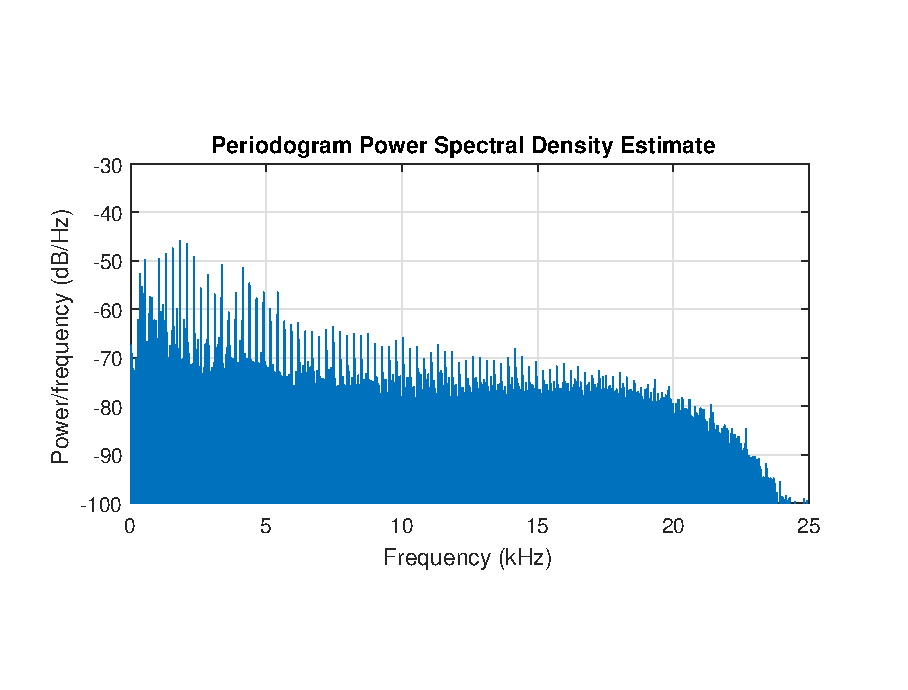
\includegraphics[trim={0cm 1.6cm 0cm 2cm},clip,width=\textwidth]{img/akustisk/Periodogram_250Hz-09.eps}
    \caption{Periodogram of 250Hz recorded tone, duty cycle 09.}
    \label{fig:period_250-09}
\end{figure}
\begin{figure}[H]
    \centering
    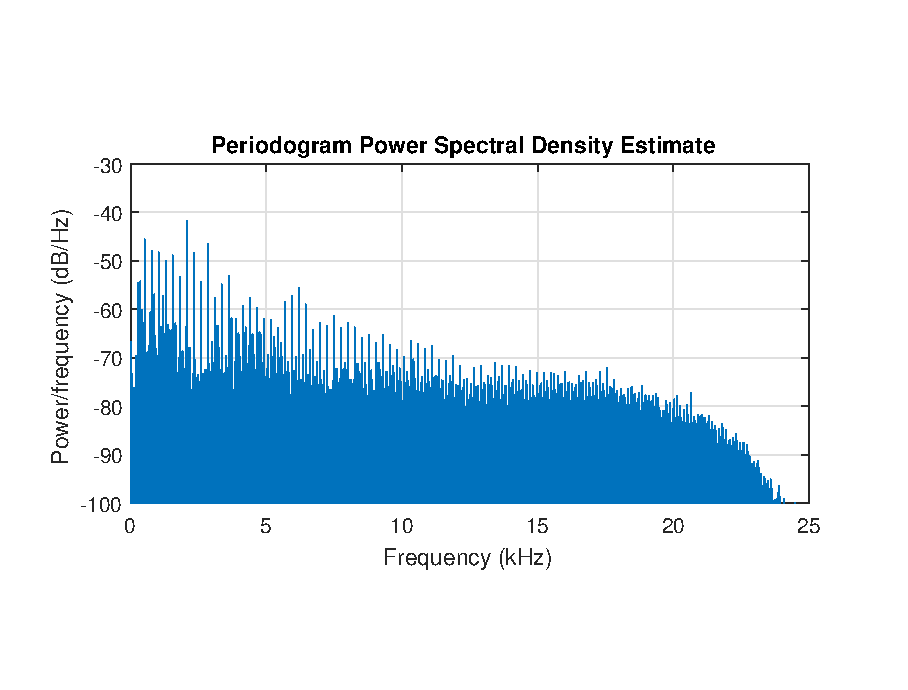
\includegraphics[trim={0cm 1.6cm 0cm 2cm},clip,width=\textwidth]{img/akustisk/Periodogram_250Hz-10.eps}
    \caption{Periodogram of 250Hz recorded tone, duty cycle 10.}
    \label{fig:period_250-10}
\end{figure}

\begin{figure}[H]
    \centering
    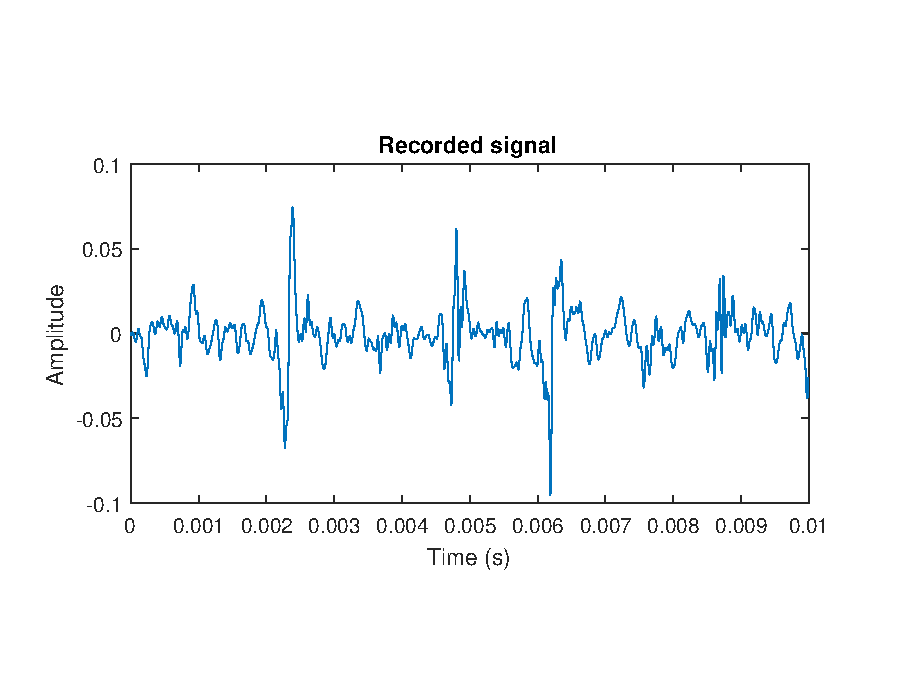
\includegraphics[trim={0cm 1.6cm 0cm 2cm},clip,width=\textwidth]{img/akustisk/Waveform_250Hz-09.eps}
    \caption{Time domain plot of 250Hz recorded tone, duty cycle 09.}
    \label{fig:appdx:wave_250-09}
\end{figure}
\begin{figure}[H]
    \centering
    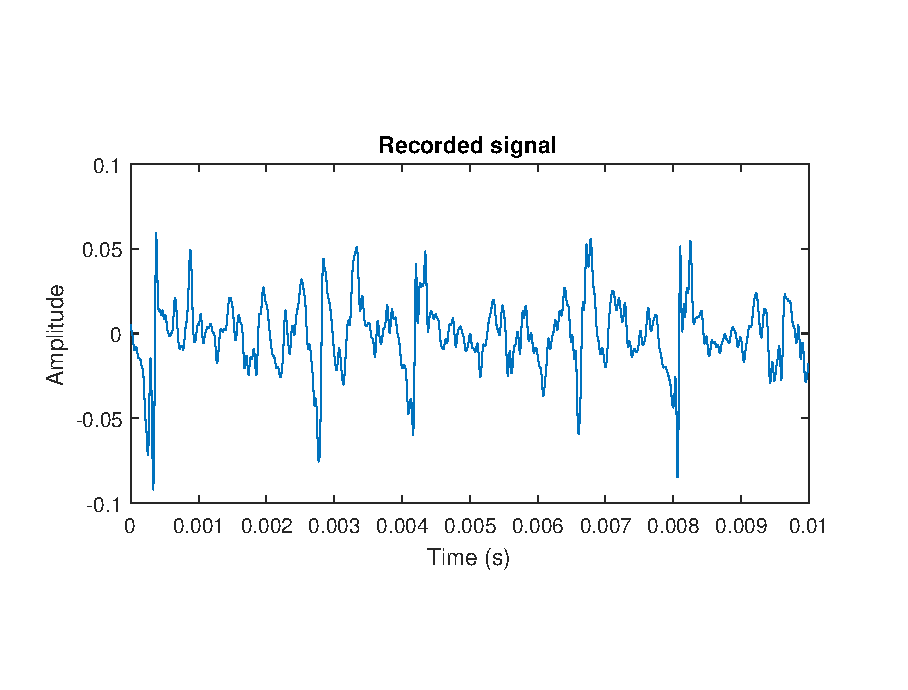
\includegraphics[trim={0cm 1.6cm 0cm 2cm},clip,width=\textwidth]{img/akustisk/Waveform_250Hz-10.eps}
    \caption{Time domain plot of 250Hz recorded tone, duty cycle 10.}
    \label{fig:appdx:wave_250-10}
\end{figure}
%%%%%%%%%%%%%%%%%%%%%%%%%%%%%%%%%%%%%%%%%%%%%%%%%%%%%%%%%%%%%%%%%%%%%%%%%%%%%%%%%%%%%%%%%%%%%%%%%%%%
\begin{figure}[H]
    \centering
    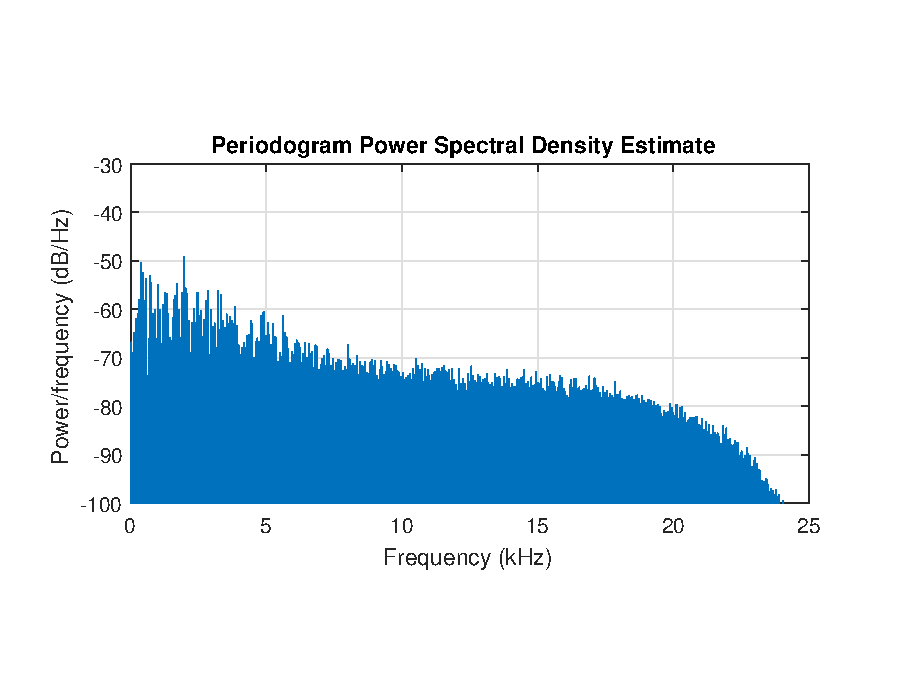
\includegraphics[trim={0cm 1.6cm 0cm 2cm},clip,width=\textwidth]{img/akustisk/Periodogram_63Hz-09.eps}
    \caption{Periodogram of 63Hz recorded tone, duty cycle 09.}
    \label{fig:period_63-09}
\end{figure}
\begin{figure}[H]
    \centering
    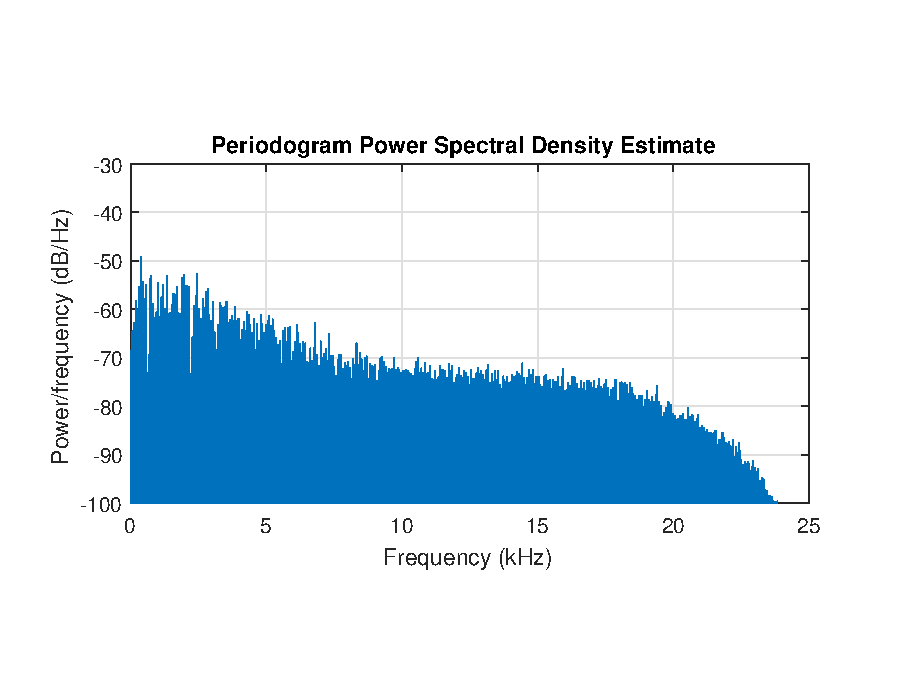
\includegraphics[trim={0cm 1.6cm 0cm 2cm},clip,width=\textwidth]{img/akustisk/Periodogram_63Hz-10.eps}
    \caption{Periodogram of 63Hz recorded tone, duty cycle 10.}
    \label{fig:period_63-10}
\end{figure}

\begin{figure}[H]
    \centering
    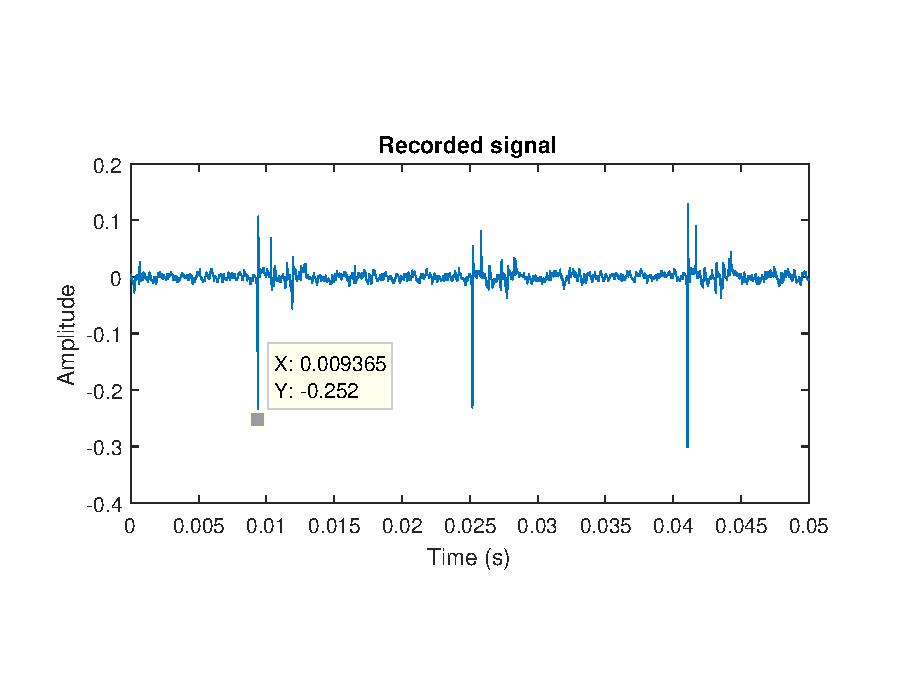
\includegraphics[trim={0cm 1.6cm 0cm 2cm},clip,width=\textwidth]{img/akustisk/Waveform_63Hz-09.eps}
    \caption{Time domain plot of 63Hz recorded tone, duty cycle 09.}
    \label{fig:appdx:wave_63-09}
\end{figure}
\begin{figure}[H]
    \centering
    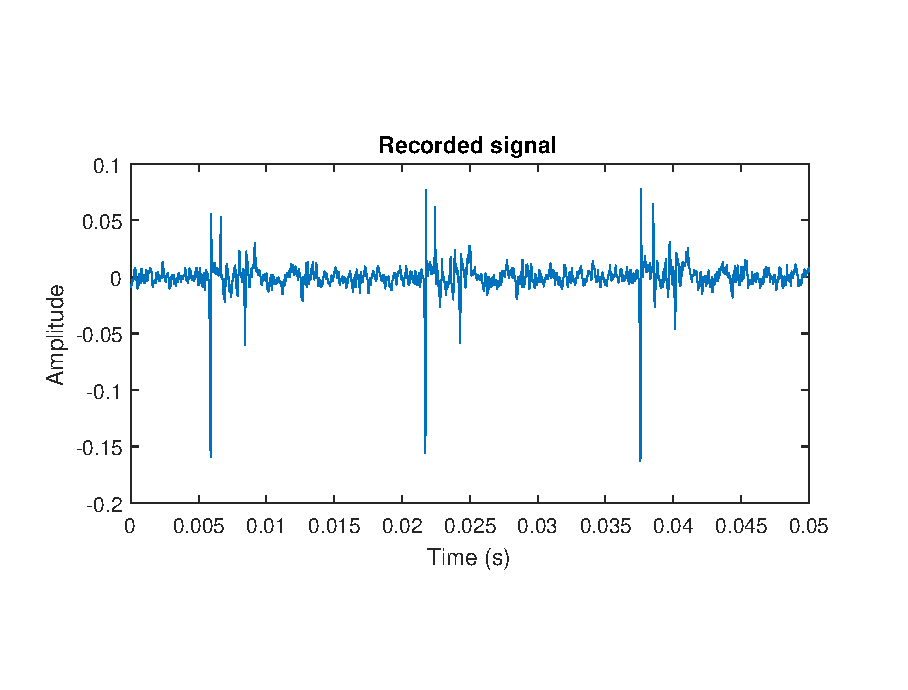
\includegraphics[trim={0cm 1.6cm 0cm 2cm},clip,width=\textwidth]{img/akustisk/Waveform_63Hz-10.eps}
    \caption{Time domain plot of 63Hz recorded tone, duty cycle 10.}
    \label{fig:appdx:wave_63-10}
\end{figure}
%%%%%%%%%%%%%%%%%%%%%%%%%%%%%%%%%%%%%%%%%%%%%%%%%%%%%%%%%%%%%%%%%%%%%%%%%%%%%%%%%%%%%%%%%%%%%%%%%%%%